\documentclass[a4paper,11pt]{article}

\usepackage[english,greek]{babel}
\usepackage[utf8]{inputenc}
\usepackage[T1]{fontenc}
\usepackage{amsmath}
\usepackage{amssymb}
\usepackage{graphicx}
\usepackage{booktabs}
\usepackage{float}
\usepackage{hyperref}
\usepackage{listings}
\usepackage{xcolor}
\usepackage[left=2.5cm,right=2.5cm,top=2.5cm,bottom=2.5cm]{geometry}

% Ρυθμίσεις για την εμφάνιση κώδικα
\definecolor{codegreen}{rgb}{0,0.6,0}
\definecolor{codegray}{rgb}{0.5,0.5,0.5}
\definecolor{codepurple}{rgb}{0.58,0,0.82}
\definecolor{backcolour}{rgb}{0.95,0.95,0.92}

\lstdefinestyle{mystyle}{
    backgroundcolor=\color{backcolour},   
    commentstyle=\color{codegreen},
    keywordstyle=\color{magenta},
    numberstyle=\tiny\color{codegray},
    stringstyle=\color{codepurple},
    basicstyle=\ttfamily\footnotesize,
    breakatwhitespace=false,         
    breaklines=true,                 
    captionpos=b,                    
    keepspaces=true,                 
    numbers=left,                    
    numbersep=5pt,                  
    showspaces=false,                
    showstringspaces=false,
    showtabs=false,                  
    tabsize=2
}

\lstset{style=mystyle}

\newcommand{\lt}[1]{\foreignlanguage{english}{#1}}

\title{1η Υποχρεωτική Εργασία \\ Στο Μάθημα <<Υπολογιστική Νοημοσύνη - Στατιστική Μάθηση>>}
\author{Όνοματεπώνυμο: Γεώργιος Κεσογλίδης \\ ΑΕΜ: 220}
\date{\today}

\begin{document}

\maketitle

\begin{abstract}
Στην παρούσα εργασία υλοποιήθηκε από το μηδέν ένας αλγόριθμος \lt{Support Vector Regression (SVR)} με χρήση της μεθόδου \lt{Stochastic Gradient Descent}. Το μοντέλο (\lt{MySVR}) συγκρίθηκε με καθιερωμένους αλγόριθμους μηχανικής μάθησης (\lt{Random Forest, Ridge, Scikit-Learn SVR}) σε δύο διαφορετικά σύνολα δεδομένων: \lt{California Housing} και \lt{Diabetes}. Η αξιολόγηση βασίστηκε σε μετρικές σφάλματος \lt{(RMSE, MAE)} και στο συντελεστή προσδιορισμού ($R^2$).
\end{abstract}

\tableofcontents
\newpage

\section{Εισαγωγή}
Η Παλινδρόμηση Διανυσμάτων Υποστήριξης (\lt{Support Vector Regression - SVR}) είναι μια ισχυρή μέθοδος επιβλεπόμενης μάθησης που στοχεύει στην εύρεση μιας συνάρτησης $f(x)$ η οποία αποκλίνει από τους πραγματικούς στόχους $y_i$ το πολύ κατά $\epsilon$, ενώ παράλληλα παραμένει όσο το δυνατόν πιο "επίπεδη".

Σε αυτή την εργασία, υλοποιήσαμε μια προσαρμοσμένη εκδοχή του \lt{SVR (MySVR}) χρησιμοποιώντας ένα νευρωνικό δίκτυο ενός επιπέδου (\lt{Dense Layer}) και βελτιστοποίηση μέσω \lt{Stochastic Gradient Descent (SGD).}

\section{Μεθοδολογία και Υλοποίηση}
Η υλοποίηση πραγματοποιήθηκε σε \lt{Python} 3.12.4 σε περιβάλλον \lt{Jupyter Notebook}.

\subsection{Συνάρτηση Απώλειας (\lt{Epsilon Insensitive Loss})}
Για την εκπαίδευση του \lt{SVR} χρησιμοποιήθηκε η συνάρτηση απώλειας \lt{Epsilon-Insensitive}, η οποία αγνοεί σφάλματα μικρότερα από ένα κατώφλι $\epsilon$:
\begin{equation}
L_\epsilon(y, \hat{y}) = \max(0, |y - \hat{y}| - \epsilon)
\end{equation}
Η παράγωγος αυτής της συνάρτησης, η οποία είναι απαραίτητη για τον αλγόριθμο \lt{SGD}, ορίζεται ως:
\[
\frac{\partial L}{\partial \hat{y}} = \begin{cases} 
-1 & \text{αν } y - \hat{y} > \epsilon \\
1 & \text{αν } y - \hat{y} < -\epsilon \\
0 & \text{διαφορετικά}
\end{cases}
\]

\subsection{Αρχιτεκτονική Δικτύου (\lt{Dense Layer})}
Η κλάση \lt{Dense} υλοποιεί ένα πλήρως συνδεδεμένο επίπεδο.
\begin{itemize}
    \item \textbf{\lt{Forward Pass}}: Υπολογίζει την έξοδο $\hat{y} = XW + b$.
    \item \textbf{\lt{Backward Pass}}: Υπολογίζει τις κλίσεις (\lt{gradients}) για τα βάρη $W$ και την πόλωση $b$ χρησιμοποιώντας τον κανόνα της αλυσίδας.
\end{itemize}

\subsection{Βελτιστοποιητής (\lt{SGD with Weight Decay})}
Για την ενημέρωση των βαρών χρησιμοποιήθηκε ο \lt{Stochastic Gradient Descent} με προσθήκη \lt{L2 Regularization} (μείωση βαρών - \lt{weight decay}) για την αποφυγή υπερπροσαρμογής (\lt{overfitting}).
Ο κανόνας ενημέρωσης είναι:
\begin{equation}
W_{t+1} = W_t \cdot (1 - \eta \lambda) - \eta \nabla L
\end{equation}
όπου $\eta$ ο ρυθμός μάθησης και $\lambda$ η παράμετρος \lt{weight decay}.

\section{Πειραματική Διαδικασία}

\subsection{Προετοιμασία Δεδομένων}
Χρησιμοποιήθηκαν δύο σύνολα δεδομένων από τη βιβλιοθήκη \lt{scikit-learn}:
1. \textbf{\lt{California Housing}}: Πρόβλεψη αξίας κατοικιών (20,640 δείγματα, 8 χαρακτηριστικά).
2. \textbf{\lt{Diabetes}}: Πρόβλεψη εξέλιξης της νόσου (442 δείγματα, 10 χαρακτηριστικά).

Εφαρμόστηκε η εξής στρατηγική προεπεξεργασίας:
\begin{itemize}
    \item \textbf{Διαχωρισμός}: 60\% Εκπαίδευση, 40\% Έλεγχος.
    \item \textbf{Κανονικοποίηση (\lt{Scaling})}: Εφαρμόστηκε \lt{StandardScaler} ($z = \frac{x - \mu}{\sigma}$) τόσο στα χαρακτηριστικά εισόδου $X$ όσο και στον στόχο $y$. Αυτό είναι κρίσιμο για τη σύγκλιση του SVR.
\end{itemize}

\subsection{Μοντέλα Σύγκρισης}
Το \lt{MySVR} συγκρίθηκε με τα εξής μοντέλα:
\begin{itemize}
    \item \lt{SVR (Linear \& RBF Kernel)} της \lt{scikit-learn}
    \item \lt{Ridge Regression} (Γραμμικό μοντέλο με \lt{L2} ομαλοποίηση)
    \item \lt{Random Forest Regressor} (Μη γραμμικό μοντέλο συνόλου)
\end{itemize}

\section{Αποτελέσματα}

\subsection{\lt{California Housing Dataset}}
Στον Πίνακα \ref{tab:california} παρουσιάζονται τα αποτελέσματα για το σύνολο δεδομένων \lt{California Housing}. Το \lt{Random Forest} πέτυχε την καλύτερη επίδοση, αναδεικνύοντας τη μη γραμμική φύση του προβλήματος. Το \lt{MySVR} (το οποίο είναι γραμμικό στην τρέχουσα υλοποίηση) είχε παρόμοια επίδοση με το \lt{Ridge Regression}.

\begin{table}[H]
\centering
\caption{Αποτελέσματα στο \lt{California Housing}}
\label{tab:california}
\begin{tabular}{lcccc}
\toprule
\textbf{Μοντέλο} & \textbf{\lt{RMSE}} & \textbf{\lt{MAE}} & \textbf{$R^2$ \lt{Score}} & \textbf{Χρόνος \lt{(ms)}} \\
\midrule
\lt{Random Forest} & 0.5216 & 0.3428 & 0.7967 & 864 \\
\lt{SVR (RBF)} & 0.6325 & 0.4484 & 0.7012 & 1986 \\
\lt{Ridge} & 0.7373 & 0.5337 & 0.5940 & 1 \\
\textbf{\lt{MySVR (Custom)}} & \textbf{0.7457} & \textbf{0.5211} & \textbf{0.5847} & \textbf{129386} \\
\lt{SVR (Linear)} & 2.1943 & 1.9346 & -2.5967 & 668 \\
\bottomrule
\end{tabular}
\end{table}

\begin{figure}[H]
    \centering
    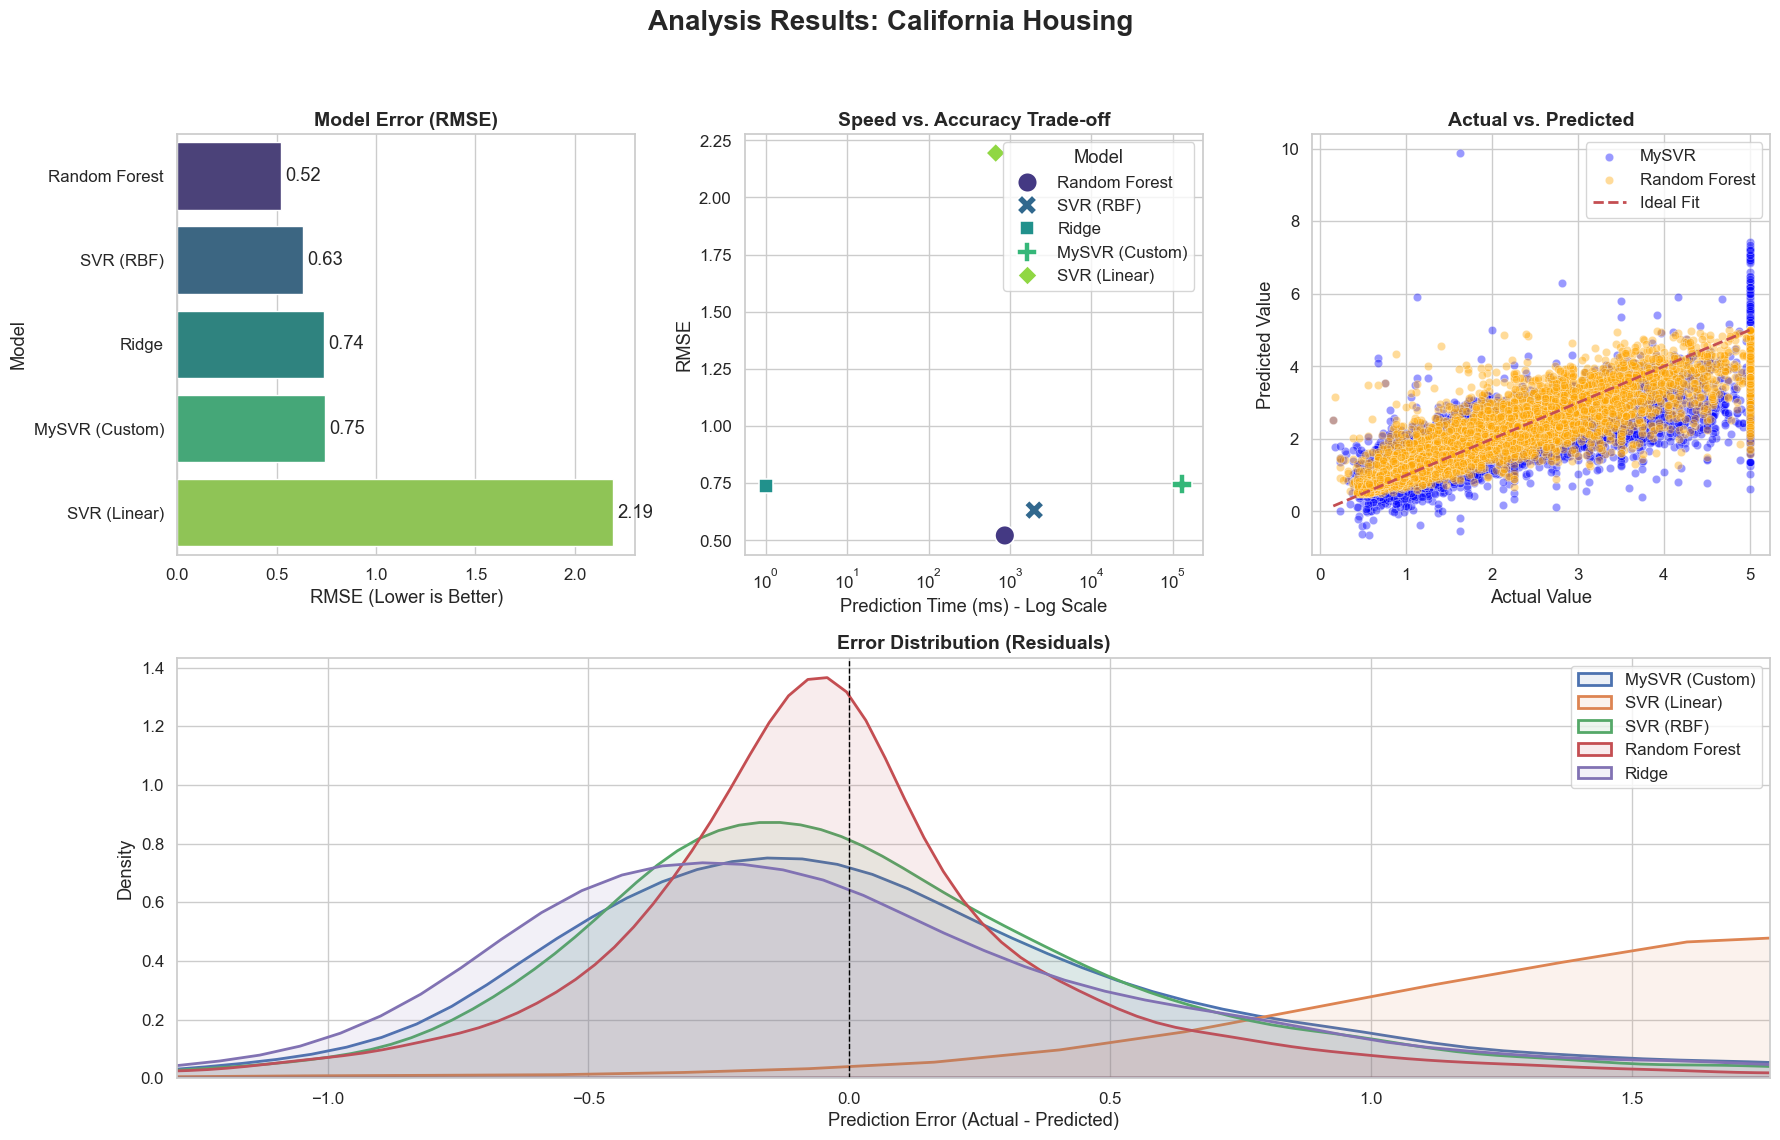
\includegraphics[width=0.8\textwidth]{california_plot.png} 
    \caption{Γραφική απεικόνιση αποτελεσμάτων για το \lt{California Housing.} (α) Σύγκριση \lt{RMSE}, (β) Πραγματικές vs Προβλεπόμενες τιμές.}
    \label{fig:california}
\end{figure}

\subsection{\lt{Diabetes Dataset}}
Στον Πίνακα \ref{tab:diabetes} βλέπουμε τα αποτελέσματα για το σύνολο δεδομένων Diabetes. Εδώ, το πρόβλημα είναι πιο γραμμικό. Το \lt{MySVR} πέτυχε επίδοση \lt{(RMSE: 53.74)} εξαιρετικά κοντά στο \lt{SVR Linear} της βιβλιοθήκης \lt{(RMSE: 53.63)} και στο \lt{Ridge (RMSE: 53.31)}, αποδεικνύοντας την ορθότητα της υλοποίησης.

\begin{table}[H]
\centering
\caption{Αποτελέσματα στο \lt{Diabetes}}
\label{tab:diabetes}
\begin{tabular}{lcccc}
\toprule
\textbf{Μοντέλο} & \textbf{\lt{RMSE}} & \textbf{\lt{MAE}} & \textbf{$R^2$ \lt{Score}} & \textbf{Χρόνος \lt{(ms)}} \\
\midrule
\lt{SVR (RBF)} & 52.6987 & 40.9211 & 0.5253 & 3 \\
\lt{Ridge} & 53.3114 & 42.5680 & 0.5142 & 0 \\
\lt{SVR (Linear)} & 53.6305 & 42.6496 & 0.5084 & 5 \\
\lt{\textbf{MySVR (Custom)}} & \textbf{53.7446} & \textbf{42.7115} & \textbf{0.5063} & \textbf{2871} \\
\lt{Random Forest} & 54.7900 & 43.6450 & 0.4869 & 86 \\
\bottomrule
\end{tabular}
\end{table}

\begin{figure}[H]
    \centering
    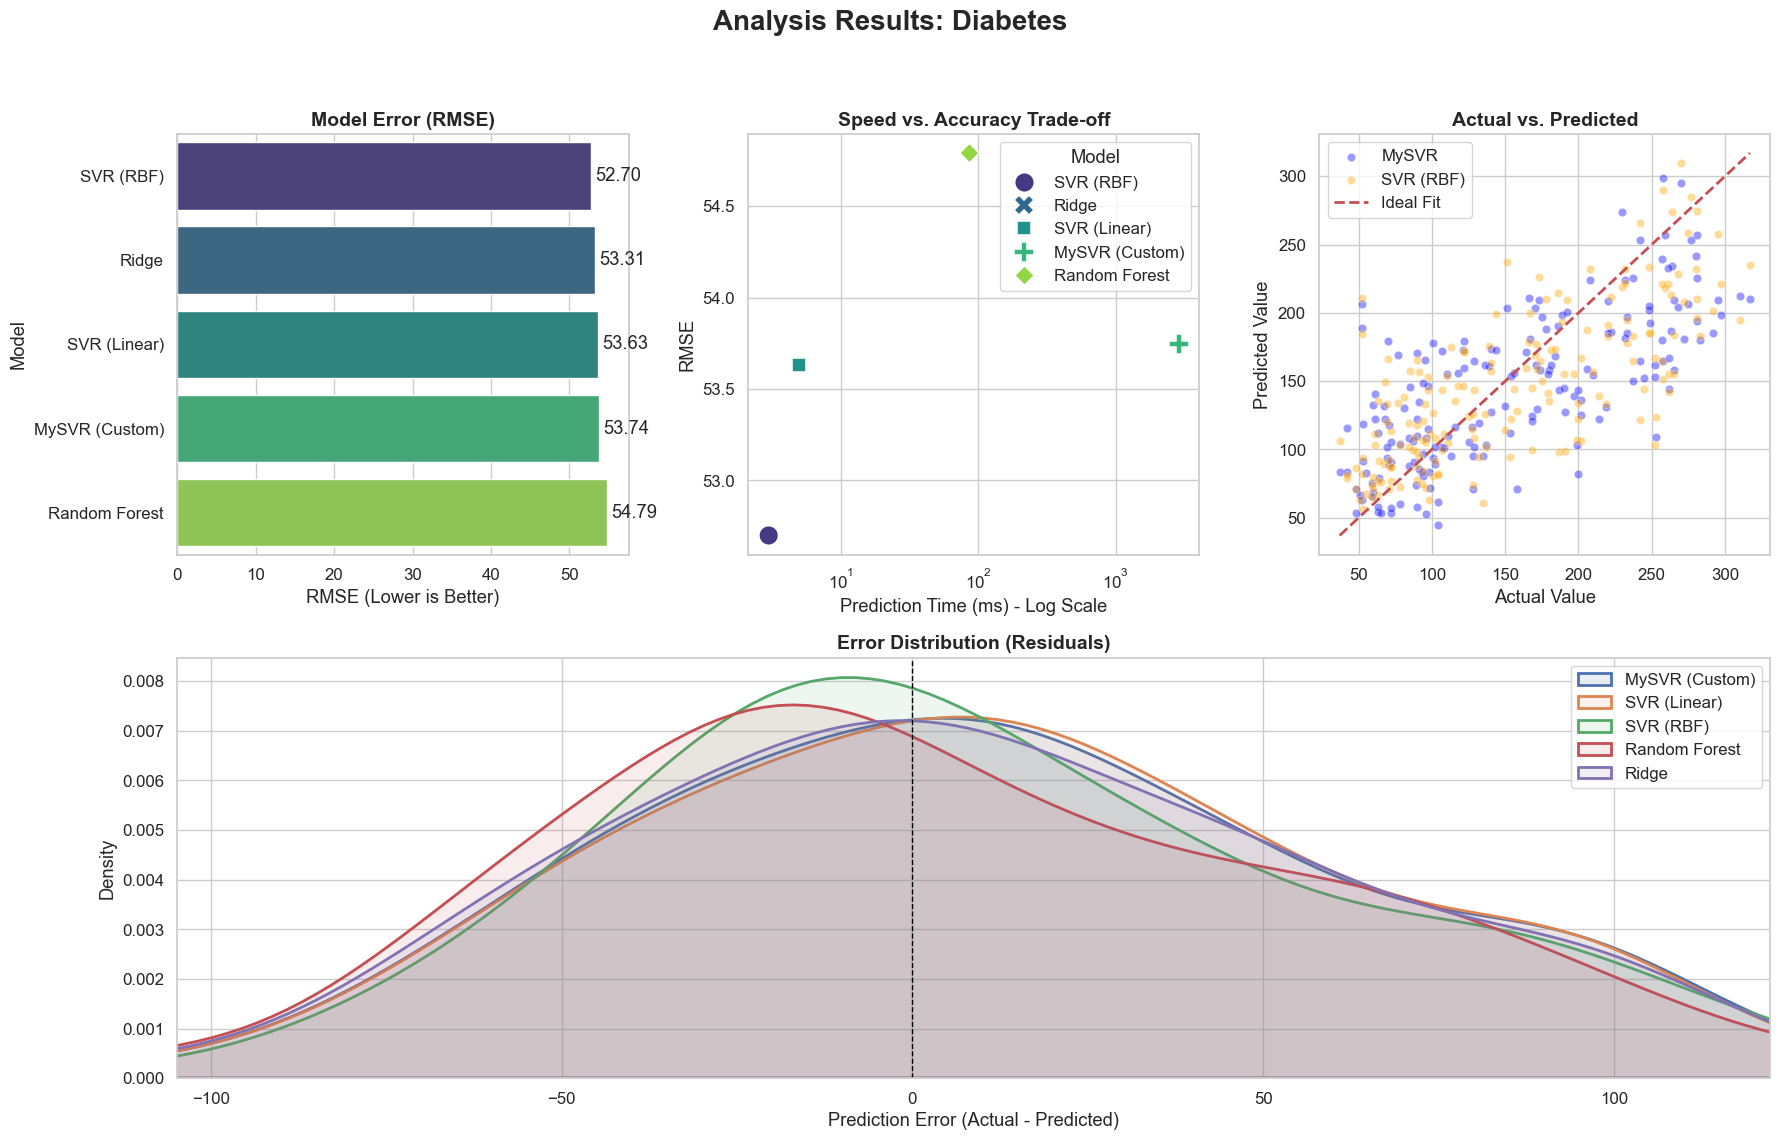
\includegraphics[width=0.8\textwidth]{diabetes_plot.png} 
    \caption{Γραφική απεικόνιση αποτελεσμάτων για το \lt{Diabetes.} (α) Σύγκριση \lt{RMSE}, (β) Πραγματικές vs Προβλεπόμενες τιμές.}
    \label{fig:diabetes}
\end{figure}

\section{Συμπεράσματα}
Η υλοποίηση του \lt{MySVR} ήταν επιτυχής καθώς κατάφερε να προσεγγίσει την απόδοση των βελτιστοποιημένων βιβλιοθηκών σε γραμμικά προβλήματα (όπως το \lt{Diabetes}).
\begin{itemize}
    \item Η κανονικοποίηση του στόχου ($y$) αποδείχθηκε καθοριστική για τη σύγκλιση του αλγόριθμου.
    \item Ο χρόνος εκτέλεσης της \lt{Python} υλοποίησης \lt{(MySVR)} είναι σημαντικά μεγαλύτερος από τις \lt{C-optimized} υλοποιήσεις του \lt{scikit-learn}, κάτι που είναι αναμενόμενο.
    \item Σε μη γραμμικά δεδομένα \lt{(California Housing)}, το \lt{RBF kernel} και τα \lt{Random Forests} υπερέχουν ξεκάθαρα έναντι των γραμμικών προσεγγίσεων.
\end{itemize}

\end{document}